% Etapes de conception, insister sur :
% architecture, choix, caractéristiques finales du système implanté

Nous allons présenter dans cette partie les principales étapes de conception
de notre réseau de neurones en détaillant tous les blocs réalisés et les choix
faits a propos de leur architecture.

\subsection{Programme de référence}
% Description du programme de référence en C, de l'utilisation de la base
% de données MNIST, du script en Python, des tableaux contenant les données,
% du taux d'erreur.
Le programme de référence implémente le même réseau de neurone que notre IP
mais directement en C. On peut ainsi l'executer sur un PC ou un micro-processeur 
et comparer les résultats avec l'implémentation réelle sur FPGA.

\subsubsection{L'algorithme}

\begin{algorithm}
	\SetAlgoLined
	\For {$f \leftarrow 0$ \KwTo $frames$} {
		$out1[neurons] \leftarrow 0$\;
		$out2[10] \leftarrow 0$\;
		\For {$r \leftarrow 0$ \KwTo $rows$} {
			\For {$c \leftarrow 0$ \KwTo $columns$} {
				\For {$n \leftarrow 0$ \KwTo $neurons$} {
					$out1[n] \leftarrow out1[n] + \texttt{get\_pixel(}f, r, j\texttt{)} \times w1[n][r][c]$\;
				}
			}
		}
		\For {$n \leftarrow 0$ \KwTo $neurons$} {
			$out1[n] \leftarrow \texttt{cut(}out1[n]\texttt{)}$\;
			$out1[n] \leftarrow out1[n] + b1[n]$\;
		}
		\For {$n \leftarrow 0$ \KwTo $neurons$} {
			\For {$i \leftarrow 0$ \KwTo $9$} {
				$out2[i] \leftarrow out2[i] + out1[n] \times w2[i][n]$\;
			}
		}
		\For {$i \leftarrow 0$ \KwTo $9$} {
			$out2[n] \leftarrow \texttt{cut(}out2[n]\texttt{)}$\;
			$out2[n] \leftarrow out2[n] + b2[n]$\;
		}
		$\texttt{assert(max(}out2\texttt{)} == \texttt{get\_label(}f\texttt{))}$\;
	}
	\caption{Boucle de calcul principal du réseau de neurone logiciel}
	\label{fig:soft_nn}
\end{algorithm}

L'algorithme~\ref{fig:soft_nn} page~\pageref{fig:soft_nn} implémente un réseau de neurones à deux étages.
Chaque étage réalise des multiplications et accumulations pour chaque pixel de
chaque image avec des poids, spécifiques à chaque neurone. Après chaque étage,
le résultat de chaque neurone est additionné avec une constante.

\subsubsection{Les données à traiter dans le réseau}

La configuration actuelle de ce réseau de neurone est adaptée pour la
reconnaissance de chiffres manuscrits de la base de données MNIST. Une image
en entrée ($28 \times 28$ pixels) correspond à un chiffre manuscrit de 0 à 9.
Le but de ce réseau de neurone est de reconnaître et d'identifier le chiffre
d'une image. Pour une image donnée, le chiffre identifié par le réseau correspond
au numéro du neurone de sortie qui a la plus grande valeur. \\
Dans ce modèle logiciel, les pixels sont encodés sur un octet, les poids et les
constantes sont sur 2 octets. Afin que dans le pire cas, aucune information ne
soit perdue lors de l'accumulation aux différents étages, on réalise cette opération sur
8 octets. Cependant, on ne doit en sélectionner que 2 sur les 8 pour effectuer l'ajout de la constante
sur des nombres de même taille et envoyer ce résultat au deuxième niveau. C'est
le rôle de la fonction \texttt{cut} qui permet de passer de 64 à 16 bits tout
en conservant le signe. Afin de choisir le bon masque, nous avons effectué
plusieurs essais et gardé celui qui menait au plus bas taux d'erreur (table
\ref{fig:masques} page~\pageref{fig:masques}).

\begin{table}[h!]
\centering
	\begin{tabular}{| l | l |}
	\hline
	Masque & Taux d'erreur \\ \hline
	0xFFFF0000 & 91.30 \\ \hline
	0x0FFFF000 & 91.30 \\ \hline
	0x03FFFC00 & 83.10 \\ \hline
	0x01FFFE00 & 28.80 \\ \hline
	0x00FFFF00 & 11.60 \\ \hline
	0x007FFF80 & 16.30 \\ \hline
	0x000FFFF0 & 90.70 \\ \hline
	\end{tabular}
	\caption{Essais de différents masques et leur taux d'erreur}
	\label{fig:masques}
\end{table}

Ainsi, nous masquons les résultats du premier niveau avec le masque sur 64 bits
\texttt{0x00FFFF00} (les bits de poids fort ne sont pas représentés ici) puis
nous effectuons un décalage pour garder uniquement ces bits, de 8 à 23. Ce
résultat nous a aussi aidé à effectuer le même masque et décalage dans notre
réseau de neurones matériel.

\subsubsection{Mise en forme des données MNIST}

Les poids des neurones et les constantes des étages de recodage
pour l'application MNIST, que nous utilisons dans
le logiciel de référence et dans notre IP nous ont été fournis au début du projet
sous forme de fichier texte où sont présentes toutes les données, séparées par
des virgules, et où chaque ligne correspond à un neurone. Un script Python nous
a permis d'analyser ces fichiers pour récupérer les données utiles et de les
replacer dans un unique fichier créé \texttt{net.c} avec les définitions de
4 tableaux d'entiers. Ce fichier est inclus et compilé dans le logiciel de référence et
pour le logiciel embarqué; ainsi les poids et les constantes sont
facilement accessibles depuis le logiciel. \\
Concernant les images, nous les avons récupérées à partir du site
officiel MNIST \linebreak (\texttt{yann.lecun.com/exdb/mnist/}) sous forme de fichiers
binaires où 1000 images de taille $28 \times 28$ pixels sont représentées comme
des tableaux d'octets en C. Un autre fichier binaire nous permet de connaître
le résultat, c'est-à-dire le digit, de chacune de ces images afin de comparer le
résultat de notre réseau de neurones avec le résultat attendu.
Les fonctions \texttt{get\_pixel} et \texttt{get\_label} permettent d'obtenir
facilement ces informations depuis le logiciel.

\subsubsection{Les résultats}

Les résultats du logiciel de référence en sortie de chacun des niveaux nous
sont utiles pour les comparer avec ceux de notre IP et s'assurer que les calculs
sont justes pour la classification des images MNIST. On s'attend à trouver
un même taux d'erreur minimal ($11.60\%$) car les configurations sont identiques
mais un calcul beaucoup plus rapide de toutes les images.
% TODO: compléter en fonctions des derniers résultats

\subsection{IP du réseau de neurones}

\begin{figure}[h!]
	\begin{center}
		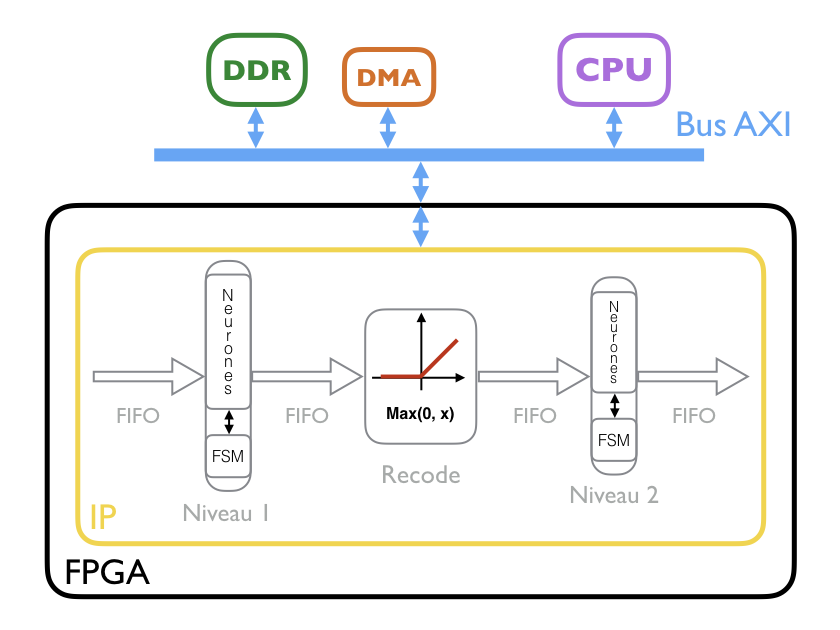
\includegraphics[scale=0.4]{NNSchema}
		\label{fig:NNSchema}
		\caption{Schéma de l'IP réseau de neurones dans son environnement }
	\end{center}
\end{figure}

\subsubsection{Le neurone}
	Le neurones est l'élément de base de notre réseau.
	C'est donc la première chose que nous avons implémenter.
	Pour faire cela, nous avons pensé le neurone en terme de
	fonctionnalités uniquement.
	Nous allons donc décrire ici la façons dont nous avons conçu un neurone. 
	Un neurones a deux modes de fonctionnement.
	Le premier est le mode de chargement des poids en mémoire, le second
	est le mode de calculs.

	\subsubsection{Le mode de chargement des poids}
	Pour permettre aux neurones d'accomplir leur rôle principale, il faut que chaque neurone ai
	accès à leur poids. Etant donné que chaque neurone doit disposer de ces propres poids
	(identiques pour une application donnée et donc pour une grandes quantité d'images)
	il est donc préférable que chaque neurone les mémorise. Afin d'accomplir cela,
	les neurones reçoivent une adresse (numero du poids à mémoriser) ainsi qu'un poids.
	Ainsi, un neurones peut mémorisent le poids présent sur son entrée dans
	sa BRAM à l'adresse reçue à condition que ce neurones possède le {\em token} de
	configuration et qu'il reçoive le signal lui indiquant qu'un poids est présent sur son entrée.\\
	Le token de configuration est passé de neurones en neurones
	sur ordre du signal de contrôle pour qu'ils se configurent les uns après les autres.
	Vous trouverez une illustration de ce fonctionnement en
	figure~\ref{fig:N_poids} page~\pageref{fig:N_poids}.
	\begin{figure}[h!]
		\begin{center}
			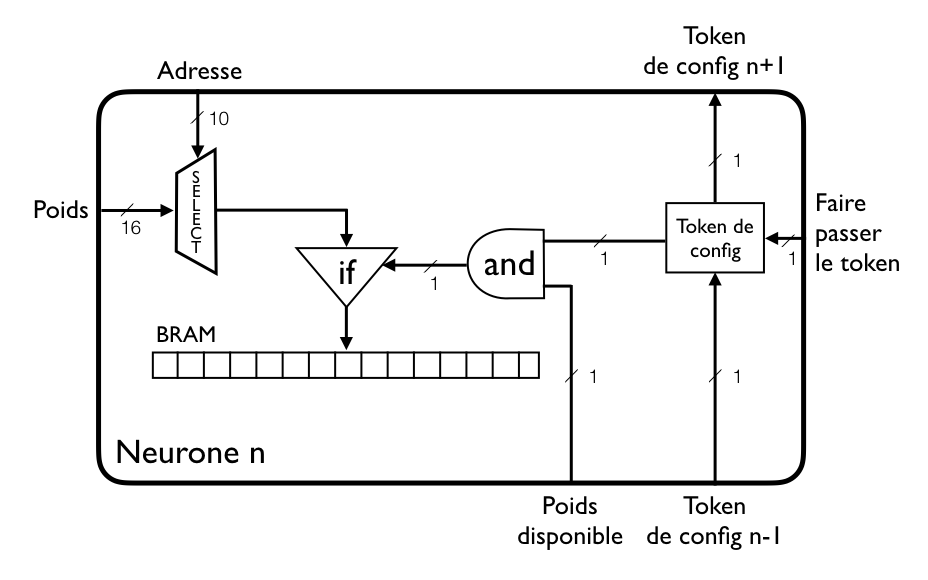
\includegraphics[scale=0.4]{N_poids}
			\caption{Schéma fonctionnel de l'implémentation du neurone en mode de configuration}
			\label{fig:N_poids}
		\end{center}
	\end{figure}

	\subsubsection{Le mode de calcul}
	\begin{figure}[h!]
		\begin{center}
			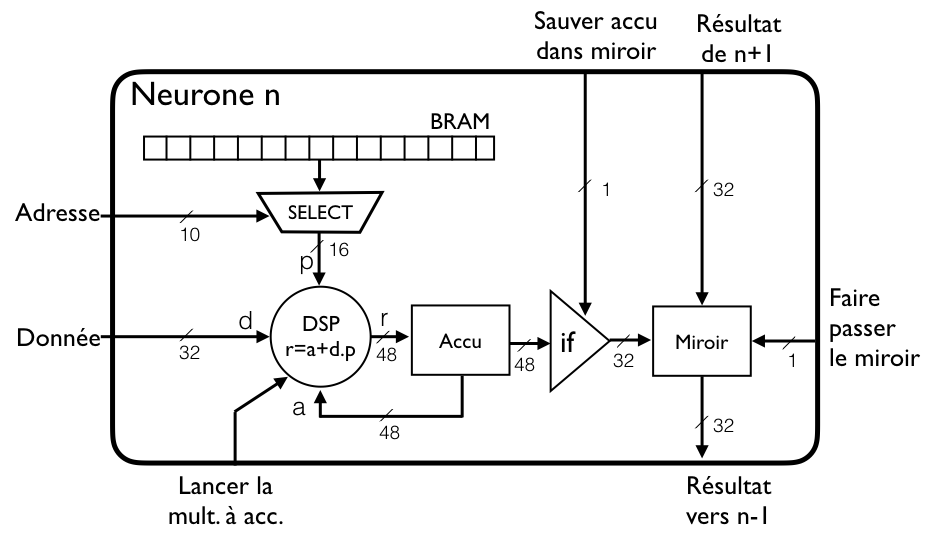
\includegraphics[scale=0.4]{N_calcul}
			\caption{Schéma fonctionnel de l'implémentation du neurone en mode de calcul}
			\label{fig:N_calcul}
		\end{center}
	\end{figure}

\subsubsection{La machine à états (FSM) du niveau de neurones}
\subsubsection{Le niveau de neurones}
\subsubsection{L'étage de recodage}

\subsection{Logiciel de commande}
Le logiciel de commande est le logiciel embarqué sur la carte, qui s'execute
sur processeur ARM et qui permet de configurer notre réseau de neurones avec
les poids et les constantes choisies, de lancer les calculs avec les valeurs
voulues et de récupérer les résultats. Il s'écrit en C et interface avec
l'utilisateur grâce à la liaison série (composant UART). Le squelette de base
était déjà disponible avec toutes les fonctions nécessaires, et le code était
écrit pour la configuration d'un niveau de neurone, l'envoi d'images simples et
la récupération des résultats.
Les données
concernant les poids, les constantes, les images et les paramètres (taille d'une
image, nombre de neurones à chaque niveau, nombre d'images) étaient toutes notées
dans un fichier (\texttt{dataset.h}). Nous avons gardé ce fonctionnement pour la
majeur partie de notre projet car il nous a permis de tester facilement notre
IP pour des images de petites tailles, des niveaux de neurones avec très peu
de neurones (3) et de configurer facilement les pixels des images et les poids
choisis pour connaître les résultats attendus et comparer avec ceux de notre IP.
Par la suite, nous avons repris les mêmes données MNIST que pour le logiciel de
référence afin de tester une application réelle. \\
% à finir HUGUES

\subsection{Caractéristiques finales du système implanté}























